\part{Philosophy of Computation}

\vspace{4mm}
\begin{displayquote}
    \textit{We're presently in the midst of a third intellectual revolution. The first came with Newton: the planets obey physical laws. The second came with Darwin: biology obeys genetic laws. In today’s third revolution, we're coming to realize that even minds and societies emerge from interacting laws that can be regarded as computations. \textbf{Everything is a computation.}}
    \vspace{2mm}
    \begin{flushright}
        ---Rudy Rucker
    \end{flushright}
\end{displayquote}
\vspace{4mm}

\textit{Computation} is an essential part of being human. Just as we act on our perceptions, feel our emotions, and daydream in our imaginations, we also compute with our \textit{reason} in order to find answers to the questions we have about life. \\

One can describe computation in a variety of ways. Some are poetic, others are more formal, and many we will discuss at length. In doing so, we will generally flow from poetry to formality, starting with broad statements and colorful examples and progressing toward a more sophisticated understanding. For now, we will say that computation is a process which resolves \textit{uncertainty}. \\

In his \textit{Theogony}, the Ancient Greek poet Hesiod (fl. 750 BCE) depicts a fascinating uncertainty called Chaos: a vast nothingness that preceded the creation of the Universe. From this void emerged the primordial deities, personifications of nature who gave life to the Titans and, by extension, to the Olympian gods. Curiously, the modern definition of chaos has nearly inverted. Now, one might say that a situation is chaotic if there is \textit{too much} going on. Despite their great conceptual difference, these meanings share a common property: they both evoke \textit{confusion}. \\

This place in which we find ourselves may indeed be post-Chaos, but confusion remains a familiar state for us. In fact, it is our natural state. We come into life confused about everything---crying, open-eyed in reaction to how much is going on around us. Slowly, we figure a few things out. Later, we consider many things \textit{certain}. As time ticks on and we carve our separate paths in the world, the wise ones among us come to realize the true depth of this confusion. \\

Although we are initially confused, we naturally pursue an understanding of the chaos that surrounds us. We perceive the goings-on of our environment and organize them into patterns that orient us and give meaning to the disorder of our existence. This is the crux of computation. It is the structured manipulation of \textit{data} into \textit{information} for the purpose of acquiring \textit{knowledge}. It shines a light into the darkness we call home. \\

These terms---\textit{data}, \textit{information}, and \textit{knowledge}---are broad enough to apply to a variety of systems. In fact, they appear in nearly every academic field and certainly within those that strive for objectivity. One can have data on, information about, and knowledge of anything that can be observed or experienced. As such, it is difficult to confine these terms to short and tidy definitions that are both rigorous and free of controversy. We will have to settle then for a long, pragmatic discussion. \\

Still, we must start somewhere. For example, you already have an idea of what information is, and it is likely that your intuition is broadly correct: information is a thing that tells you something. As we dive into more and more abstract topics, do not hesitate to, in this way, fall back on your existing vocabulary for support. A word used technically is more precise than the same word used casually, but the gist of it all is often the same. Or, at least, there is often some sense in which one reflects the other, like concepts linked in a good simile. \\

Recall the usual context in which technical language is born. A \textit{pattern} or \textit{phenomenon} is observed by a community, and it becomes the subject of casual discourse. It may even be a widespread concept that is discussed by society at large. Accordingly, the phenomenon is given an \textit{informal definition} and a \textit{name} (or, perhaps, many names). Interested theoreticians then formalize it; they describe its \textit{form} in unambiguous terms. They give it a \textit{formal definition} and bestow a more permanent name upon it, either one used previously or something new that, in the namers' opinion, better conveys the idea. In the latter case, the new term is disseminated throughout the community and perhaps to the wider public, where it may either replace or coexist with previous informal terms. Regardless, the namers must reach outside of the formalisms of their field to find a word from an informal, natural language that captures the essence of their abstract thought. \\

This is the beauty of a good piece of jargon: such a word will, to an amateur, shed a shallow but wide light into the vast space of an idea, but it will also illuminate the whole shebang in the eyes of an expert, evoking in its concise informality all that he or she has previously learned on the subject. In the spirit of this principle, our three words are defined softly below to act now as beacons in the dark of our ignorance and later as shining summaries of our hard-earned understanding: \\

\begin{displayquote}
    \textbf{Data} (sing. \textbf{datum}) are pieces of information that are meaningless when considered separately. They are observable lacks of uniformity in reality, each of which may be represented by a symbol that conveys its particular difference from the norm. \\~\\
    \textbf{Information} is an ordered arrangement of data that has the potential to convey something meaningful. The data are arranged such that the information as a whole complies with the grammar of a language that can, in theory, be understood. \\~\\
    \textbf{Knowledge} is an understanding of information that emerges given proper interpretation and purposeful thought. It is usually associated with truth and may be considered a body of true beliefs. \\
\end{displayquote}

The journey to an honest appreciation of these terms will be an arduous one, and subtly so, as it will require an open mind and an ample store of time set aside for the contemplation. Nevertheless, walking that inner path is unquestionably worth the cost when one considers how pervasive these concepts truly are. They can describe any event, including those that occur in computers as they run their software and in brains as they continuously perceive and conceive of their own respective conscious experiences. This chapter explores Man's longstanding interest in these scraps of reality: our inquiry into the smallest details of Nature; our concretization of abstract thought through language, signage, and code; our distillation of human reason into mechanical rulesets. \\

There is a fourth word---\textit{wisdom}---but it is even harder to pin down than the previous three. It is a lofty word---so lofty that it is difficult to say anything about it without sounding like a proselytizer. Its utterance conjures up images of ashen-haired, big-bearded men in togas or robes, speaking of grandiose things or passing time in peaceful admiration of the world. It has no formal definition because its form is unknown, close enough to touch momentarily but always out of reach. Furthermore, it is bound to messy human concerns like emotions, morals, and purpose. How, then, could wisdom be relevant to the study of something as well-defined as computation? \\

\chapter{Cognitive Ontology}

\vspace{4mm}
\begin{displayquote}
    \textit{The first rule is to keep an untroubled spirit. The second is to look things in the face and know them for what they are.}
    \vspace{2mm}
    \begin{flushright}
        ---Marcus Aurelius
    \end{flushright}
\end{displayquote}
\vspace{4mm}

Dark turns into light. A boundless zephyr of blurs. You see. You hear. You \textit{feel}. The knife-edge of experience materializes, and you step out onto it. It cuts you, and there is no thought---only sensation. Air kissing skin and turbulent color. Sonic frenzy and the feeling of self-weight. Reality emerges raw and beams through all you are. You are lost in it all: a sailboat in a storm, a satellite adrift in space, and the rest. Indifferent, it rages on. \\

This is roughly the experience of a newborn infant. For children of a month or so, life is a sensory mayhem of little sense. They are not conscious, at least not in the way that we typically think of consciousness. They are, however, aware of their surroundings and sensitive to \textit{phenomena} (i.e. the \textit{appearances} of reality, \textit{observables}). To newborns, the world is not a system of distinct parts but an all-encompassing soup of stimuli. Their sensory organs input data that they do not understand, and they then output \textit{reflexes} honed through millions of years of natural selection. \\

This is not to say that babies are mindless. Rather, their minds are just unlike those of typical adults, which both \textit{filter} and \textit{store} information. For example, while babies and adults have similar hearing ability, babies nevertheless hear things that adults do not. This is because adults subconsciously ignore certain sounds; they may \textit{sense} the auditory data, but they do not \textit{perceive} them. This filtering process is called \textit{sensory gating}, and it inhibits any stimulus that is deemed irrelevant. Any information that is not filtered is then eligible for storage in \textit{memory}. \\

Thus, if the adult mind is like the conical beam of a flashlight, seeing far but neglecting much, the baby mind is like the radiant orb of a lantern, seeing all that is immediate but illuminating nothing deeper. These configurations are well-suited to the goals of each: the adult needs \textit{attention} to understand complex situations whereas the baby needs \textit{unrestricted perception} to acquire as much information as possible. Unburdened by categorical thought and sensory gating, babies live in the present and see the suchness of their surroundings. However, their experience is not quite the \textit{kensh\=o} of Zen---it is more like Aldous Huxley's Mind at Large or William Blake's oft-quoted metaphor, from which Huxley took the title of his first essay on psychonautics: \\

\begin{displayquote}
    If the doors of perception were cleansed every thing would appear to man as it is: Infinite. For man has closed himself up, till he sees all things thro' narrow chinks of his cavern. \\
\end{displayquote}

So it is through a great deal of concurrent filtering and learning that we come to build a cavern around ourselves. But we do not muffle our perception pointlessly---we trade it for genuine \textit{thought}. \\

\section{Upper Ontology}

There is a distinction that is sometimes made in cognitive science between a \textit{(phenomenal) P-consciousness} and an \textit{(access) A-consciousness}, the former being the sole consciousness of the baby mind, concerned only with bits of immediate, subjective experience known as \textit{qualia} (e.g. what it is like to \textit{feel} a delicate raspberry as it touches your tongue, what it is like to \textit{taste} it as you mash it between your molars, the rush of brief and unique \textit{delight} found in enjoying that \textit{particular} berry, etc.) and the latter being the dominant consciousness of the adult mind, concerned with \textit{cognitive information} (e.g. thoughts about sensory data, abstract ideas, memories of the past, plans for the future, and all things involved in \textit{mental computation}). \\

Of course, adults still have a P-consciousness---we can lose ourselves in the moment if we are willing. But ours is a boarded-up P-consciousness, largely unaware of the immense volume of all that is happening at all times. Perhaps it is only the bodhisattvas or the mystics of yore who truly come to know their infant minds again and see the P and A as they are: two \textit{modes} of a unified whole. Or perhaps, more pessimistically (and as Huxley suggests), the P in its unadulterated totality is really a kind of schizophrenic insanity, and it is only by the grace of our specialized neural hardware that we erect defenses against its sensory onslaught. Alas, the suchness of such a consciousness eludes those of us with at least one foot planted solidly on the earth. \\\\

\subsection{The Hard Problem of Consciousness}
What is it about phenomenal consciousness that is so intangible? It has been a question of interest to humanity for thousands of years and an object of formal study since Ren\'e Descartes (1596-1650) first posited the duality of \textit{mind} and \textit{body}. Inspired by the proliferation of \textit{automata} (i.e. self-operating machines) in Paris, Descartes came to suggest the extraordinary: that animals---their limbs, organs, and mannerisms---could be replicated with sufficiently complex machinery. Further, he professed that animals \textit{themselves} were machines, with bone and flesh standing in for wood and metal: \\
        
\begin{displayquote}
    It seems reasonable since art copies nature, and men can make various automata which move without thought, that nature should produce its own automata much more splendid than the artificial ones. These natural automata are the animals. \\
\end{displayquote}
        
Note that Descartes implies here that animals are "without thought." He also claimed that thoughts required a language in which rational ideas could be expressed. (Thoughts encoded in a language, however, need not be expressed outwardly; babies, for example, mentally represent ideas before learning how to render them in speech.) He also reasoned on this basis that an automaton would never be able to think because it would never be able to speak in the way that humans do---by organically producing an appropriate response to any given prompt. (Whether or not he was correct remains to be seen, though the possibility of an \textit{artificial general intelligence} does not seem quite as absurd now as it must have seemed back then.) In Descartes' view, humans are special and cannot be reduced to machinery because, unlike animals, they possess rational minds enriched with a free will that no algorithm can replicate. \\
        
Thus, Descartes championed \textit{substance dualism} (also known as \textit{Cartesian dualism}), in which all things were either fundamentally of \textit{matter (res extensa)} or of immaterial \textit{mind (res cogitans)}. He saw the human being as a union of the two disparate substances but struggled to reconcile his strict dualist views with the decidedly hybrid and experiential character of his own bodily sensations and emotions. In the sixth and final meditation of his \textit{Meditations on First Philosophy}, Descartes states that in being skeptical of his fallible senses, he understands himself to be essentially a mind, a purely thinking thing of no physical extent that is intuitively indivisible. And yet, he nevertheless \textit{feels} the qualia of his body and thus must straddle his own \textit{mind-body duality}, being, in a phrase, both flesh and not: \\
        
\begin{displayquote}
    There is nothing which this nature teaches me more expressly [nor more sensibly] than that I have a body which is adversely affected when I feel pain, which has need of food or drink when I experience the feelings of hunger and thirst, and so on; nor can I doubt there being some truth in all this. \\

    Nature also teaches me by these sensations of pain, hunger, thirst, etc., that I am not only lodged in my body as a pilot in a vessel, but that I am very closely united to it, and so to speak so intermingled with it that I seem to compose with it one whole. For if that were not the case, when my body is hurt, I, who am merely a thinking thing, should not feel pain, for I should perceive this wound by the understanding only, just as the sailor perceives by sight when something is damaged in his vessel; and when my body has need of drink or food, I should clearly understand the fact without being warned of it by confused feelings of hunger and thirst. For all these sensations of hunger, thirst, pain, etc. are in truth none other than certain confused modes of thought which are produced by the union and apparent intermingling of mind and body. \\
\end{displayquote}
        
Fast-forward to the turn of the $20^\textit{th}$ century and general confidence in the scientific method had annealed Descartes' mechanistic philosophy into full-blown metaphysical naturalism. The Modernist movement was in full swing, quantum mechanics was being formulated, mathematics was being axiomatized, and about thirty years later the greatest minds of the era would contribute to a general theory of computation. And in the 1950s, the \textit{cognitive revolution} began, and people started to think of the mind as a complex system that could be explained in terms of information and computation. It seemed like the next logical step in human progress. Like matter had been reduced to elementary particles, like water had been reduced to H$_2$O, like genes had been reduced to DNA, so too would the mind be reduced to its constituent parts. \\
        
And yet, there is also that deep feeling in us that the mind is something else. We are inclined to believe that there is something about consciousness that is incomparable to, say, a Rube Goldberg machine or a computer running a program, no matter how complex either may be. Namely, we feel that there is \textit{something that it is like to experience being}. In 1974, philosopher of mind Thomas Nagel (b. 1937) brought this idea to the attention of the burgeoning field of \textit{cognitive science} with his paper \textit{What Is It Like to Be a Bat?}, in which he states that no physicalist theory will capture the essence of the mind until we come to understand its subjective aspects: \\
        
\begin{displayquote}
    The fact that an organism has conscious experience at all means, basically, that there is something it is like to be that organism. There may be further implications about the form of the experience; there may even (though I doubt it) be implications about the behavior of the organism. But fundamentally an organism has conscious mental states if and only if there is something that it is like to \textit{be} that organism---something it is like \textit{for} the organism. We may call this the subjective character of experience. \\
\end{displayquote}
        
This "subjective character of experience" presents a major challenge to the belief that neuroscience will eventually reduce consciousness to a theory. The \textit{philosophy of mind} is then, perhaps, brazenly Postmodernist---inherently subjective and relativistic, with answers that will remain unknown to mankind in spite of its scientific progress. Nagel posits, for example, that we cannot conceive of the subjective experience of a bat because it is totally alien to our own experience. And further, he argues that it does no good to ground such an experience in greater and greater \textit{objectivity} (i.e. independence from human bias), that such first-person character is stripped away in the third-person framework of science: \\
        
\begin{displayquote}
    It will not help to try to imagine that one has webbing on one's arms, which enables one to fly around at dusk and dawn catching insects in one's mouth; that one has very poor vision, and perceives the surrounding world by a system of reflected high-frequency sound signals; and that one spends the day hanging upside down by one's feet in an attic. In so far as I can imagine this (which is not very far), it tells me only what it would be like for \textit{me} to behave as a bat behaves. But that is not the question. I want to know what it is like for a \textit{bat} to be a bat.
    \begin{center}
        \mydots
    \end{center}
    If the subjective character of experience is fully comprehensible only from one point of view, then any shift to greater objectivity---that is, less attachment to a specific viewpoint---does not take us nearer to the real nature of the phenomenon: it takes us farther away from it. \\
\end{displayquote}
        
For Nagel, this is not necessarily a death knell for any formal understanding of consciousness, but it \textit{is} a declaration of doubt in the capacity of science \textit{as we currently know it} to shed light on such matters. His qualms lie not with physicalism itself---that is, not with the assertion that mental states are fundamentally physical---but with an overconfidence that tends to come with the territory of such a mindset. His goal is to elucidate a problem: that, while it is reasonable to believe that one's mind is the result of solely the neurobiological mechanisms in one's body, it is nevertheless \textit{unreasonable}, if we accept that qualia exist and are essential to our experience, to claim that science is presently capable of capturing the subjective character of the conscious mind within its objective bounds. \\
        
In light of this issue, Nagel concludes with a call for the formulation of an "objective phenomenology," a framework in which qualia could be described independently of their experiencer's point of view. Only then could our subjective character of experience, which is so central to our conception of being human, be expressed "in a form comprehensible to beings incapable of having those experiences." As it stands, we cannot describe our seeing of red without analogy to previous experiences of seeing red, and in such terms we can only convey our meaning to those with eyes and brains like our own. And if bats could talk, they would be similarly unable to communicate their echolocational qualia to our sonar-ignorant minds. Thus, \textit{What Is It Like to Be a Bat?} is not a position piece on the nature of qualia but a declaration of agnosticism toward it: we cannot say anything objective about what we feel until we determine whether or not our feelings have objective content. \\
        
Nevertheless, Nagel is often considered a standard-bearer for \textit{property dualism}, which holds that there are two distinct kinds of properties: \textit{physical} and \textit{mental}. Unlike Cartesian dualism, this position holds that there is only one kind of substance, and, in contemporary Western philosophy, it is almost always considered physical rather than mental, an objective entity rather than a subjective one. But Nagel is particularly a standard-bearer for a variety of property dualism known as \textit{neutral monism}, which offers a middle path: that everything is composed of a neutral stuff that is neither physical nor mental. An early form of this view was put forth by the pragmatic philosopher William James (1842-1910) in his essay \textit{Does Consciousness Exist?}: \\
        
\begin{displayquote}
    My thesis is that if we start with the supposition that there is only one primal stuff or material in the world, a stuff of which everything is composed, and if we call that stuff 'pure experience,' the knowing can easily be explained as a particular sort of relation towards one another into which portions of pure experience may enter. The relation itself is a part of pure experience; one of its 'terms' becomes the subject or bearer of the knowledge, the knower, the other becomes the object known. \\
\end{displayquote}
        
So there is a particular relation $\rightarrow$, one among many, and it is called \textit{knowing}. And it relates one term $A$ to another term $B$. And we say that $A$, the knower, \textit{knows} $B$, the known: $A \rightarrow B$. And all of these---the $\rightarrow$, the $A$, the $B$, and the composed whole---are of a neutral, experiential substance. And, indeed, so it is for everything that we may perceive or conceive. The onus is placed then on the rational interpreter to determine whether a relational structure (or \textit{pattern}) of neutral elements constitutes a physical or mental property. Thus, we are pattern-scanning machines and arbiters of what is \textit{thought} and what is \textit{thing}. \\
        
Regardless of whether or not they exist, qualia are beyond our scope. \\

\subsection{The Categories of the Mind}

\textbf{Space and time} are two features of our reality. As they appear to us, the former is an expanse in three dimensions, and the latter can be thought of as an arrow that extends steadily in one dimension, from past to future. They are inextricably woven into the fabric of our experience, and yet their true nature eludes us. \\

Consider a space that contains many particles of \textit{substance}, all of which move about constantly as time goes on. Suppose that, one by one and randomly, these particles blink out of existence forever. When only one particle remains, is that which is \textit{not} the particle still considered space? Further, can we still say that this particle moves? It remains surrounded by a void, interacting and relating with nothing at all, participating in no distinguishable events. And if indeed nothing changes, does time still tick? If so, will space and time \textit{mean} anything after that last, lonely bit of matter disappears and everything becomes a uniform non-existence? \\

These are the questions that pertain to whether space and time are \textit{absolute} or \textit{relative}. If space is absolute, like a fixed three-dimensional grid that pervades the material realm, we might ask where the origin $(0,0,0)$ is. If such a location were to exist, every object and particle in the Universe would have an absolute position in three coordinates. In other words, position would be a distinguishing feature of each and every object, and it would not be defined in relation to other objects, but to this primordial \textit{center of the Universe}. \\

If space is instead relative, a conceptual origin can be placed wherever one likes. Distances can then be measured from this point. Of course, this can be done in an absolute space as well. Thus, the absolutist viewpoint commits the cardinal sins of being \textit{unobservable} and being \textit{useless}. To any human observer, a reality with absolute space would look no different than a reality with relative space---objects would not change in any way after being related to an arbitrary center. Access to these absolute positions also would not provide us with any additional information---they would just be fixed offsets of any positions measured from a relative point. \\

Perhaps then, space is is better thought of as \textit{relational} rather than \textit{objective}. Perhaps it is not a hidden grid-like object itself, but an \textit{ordering} that is composed of relations between objects. And perhaps then it is also better thought of as a product of the \textit{mind} rather than as a physical thing. That is, space may instead be an \textit{abstraction} that our minds make by estimating the relative distance between two objects and comparing it to every other potential spatial relation in our surroundings. In this view, space is simply a web of relations that is constructed by a sentient being. \\

Similarly, time may not be a hidden clock-like object, but instead a series of relative temporal intervals between \textit{events}. And if we only know that time passes because of the changes we perceive in space, it is possible that time is an abstraction as well, an ordering of events made by a sufficiently conscious mind. Furthermore, if space and time are both relational and coupled, perhaps it is better to think of them as a unified \textit{spacetime} despite our predispositions to think of them separately. \\

The philosophy of space and time is full of eternal questions about infinity, substance, void, uniformity, asymmetry, and consciousness. Comparatively, \textit{computational space and time} are simple. \\

This curiosity aside, we could also design our category system such that quantities and qualities are both considered \textit{properties} of some very general sort of thing. Philosophers have long considered the idea of a highest-level category and have ascribed a variety of names to its members: \textit{entity}, \textit{being}, \textit{thing}, \textit{term}, \textit{individual}, etc. Each carries its own subtle connotations. We will use the name \textit{object} because it is the default choice in current philosophical practice and because it has bled into the technical language of computer science with its meaning largely unchanged. \\

How general is this category of objects? Namely, are properties objects? If they are, then our system collapses to a single category, which really means that no distinctions about reality can be made at all. The category of objects thus becomes the soupy mess we are trying to escape. For now, let us assume that properties are \textit{not} objects. Instead, they are something else, and they \textit{relate} to objects in some way, giving them their characteristics. From these relations, the diversity of existence unfolds. \\

The \textbf{abstract-concrete dichotomy} classifies \textit{things} as being either \textit{abstract} or \textit{concrete}. Despite the fact that most people recognize a difference between an abstract and a concrete thing, this dichotomy does not have a universally accepted definition. That said, being abstract is often defined as being both \textit{non-spatiotemporal} and \textit{causally inefficacious}. That is, something is abstract if and only if 

\begin{enumerate}
    \item it does not exist in \textit{space} or in \textit{time} (or, alternatively, in \textit{spacetime}), and
    \item it cannot be the \textit{cause} of any \textit{effect}.
\end{enumerate}

However, one might argue that nothing is truly causally inefficacious. Indeed, if something was truly unable to cause \textit{anything}, it would not be able to affect the \textit{thoughts} of any philosopher, mathematician, or scientist for whom such an abstract thing would be of interest. And yet \textit{mathematical objects} (e.g. a number, a line, a cube, the sine function, etc.) are often considered abstract, despite the fact that they affect the thoughts of mathematicians daily, thoughts which in turn prompt concrete behavior, such as drawing diagrams. Perhaps, causal inefficacy is too strict a requirement. \\

Let us consider why one might want to refer to something that is abstract. An abstract object references \textit{properties} that many concrete, causally efficacious objects have. For example, a sphere does not exist in space or time; it is \textit{nowhere} and \textit{never}. It also does not seem capable of causing an effect in the way that, say, a ping-pong ball can. And while the abstract sphere may not have the same sort of causal efficacy as concrete spherical objects, it does have a \textit{relation} to those objects. That is, the concept of sphericality is \textit{related} to the \textit{class} of concrete objects that may be reasonably modeled as spheres. Thus, an abstract object is, at least, convenient because it can identify a class of concrete objects that is of interest by specifying relevant properties. \\

In light of recent advancements in fields like neuroscience and artificial intelligence, many believe that the human mind is nothing more than a physical system, albeit a particularly complicated one, that can be modeled mathematically like any other. So it may be that abstract objects are just interpretations of concrete electrochemical signals in our brains. Regardless,  \\

A common approach to this challenge is creating a system of \textit{categories} that partition reality at the highest level. For example, one could suggest that there is a fundamental difference between a \textit{quantity} and a \textit{quality}. If these are considered distinct categories, we can classify \textit{measurable} or \textit{countable} stuff like \textit{length}, \textit{mass}, \textit{number}, and \textit{monetary value} as quantitative and \textit{experiential} stuff like \textit{softness}, \textit{roundness}, \textit{flavor}, and \textit{beauty} as qualitative. \\

The quantity-quality distinction is a generally accepted one. However, the dichotomy is not so absolute. For example, softness is listed above as a quality. We might expect, then, that hardness is a quality. For example, rocks are hard and puppy ears are soft. But hardness is also a quantitative measurement of resistance to plastic deformation. Thus, the word \textit{hardness} can refer to both quantitative and qualitative phenomena. The categorical difference between these hardnesses, which exists independent of language, is identified through the context in which the word is used. A hardness can be measured with numbers, but it can also simply be \textit{experienced} via touch. \\

A \textbf{domain of discourse} is a set of all the things under discussion. It is also called a \textit{universe}, particularly in the field of mathematical logic. It specifies, out of all conceivable objects of study, those objects which are pertinent to the matter at hand. It gives \textit{context} to what we say. \\

A \textit{discourse} is a conversation, and its \textit{domain} is the subject of the conversation. A domain may also refer to an entire field of study, perhaps one whose conversation has been developing for thousands of years (e.g. physics, whose domain is physical reality). Each field of study has an accompanying domain of discourse, the set of objects within its purview. Working in such a field is thus akin to exploring a \textit{universe} populated with such objects. \\

As we observe the objects of a universe, we can make \textit{logical statements} about them. We can also ensure our statements are consistent by using a \textit{formal system of deduction} to prove them from a set of \textit{axioms}. And if we compile every statement that can be proven in this system---the axioms and their consequences---we will form a \textit{theory}, a set of true statements (or \textit{theorems}) that describes the universe in question. \\

The word \textit{theory} may also refer to a \textit{theory-in-progress}, a body of logical work to which theoreticians contribute. We might consider this an \textit{open theory}, a theory for which we do not have all possible knowledge. In contrast, a \textit{closed theory} is one for which we know everything there is to know. \\

Similarly, we can describe universes as open or closed. The \textit{open-world assumption} is made when we do not have complete knowledge of a system: if a statement is not known to be true (i.e. it is not a member of our theory), we do not assume anything about its truth value. This is the case for any system that is \textit{discovered}, like the various systems of nature. \\

Computational systems, however, are not discovered but \textit{designed}. Under normal conditions, it is possible to know everything that happens during a digital computation---all of the information appears in a discrete, finite space of computer memory. Thus, we are omniscient with regard to this universe and should make the \textit{closed-world assumption}: if a statement is not known to be true, it must be false. \\

The \textbf{type-token distinction} \\

\textbf{Identity} seems to be a mandatory quirk of being. It is difficult to imagine an existence in which things are not themselves. And yet, it is also difficult to define, in any meaningful way, this supposedly crucial concept. \\

The \textbf{map-territory relation} \\

% Taxonomy diagram
\begin{center}
    \resizebox{\textwidth}{!}{
        \begin{tikzpicture}[scale=0.2]
         
            %--- GRAY TREES -------------------------
            \foreach \x in {0,...,3}{
                \foreach \y in {1,...,5}{   
                    % Big dashed lines
                    \draw [gray,dashed,thick] (\x*17,0) -- ++(90+\y*15:8);
                    \draw [gray,dashed,thick] (\x*17,0) -- ++(180+\y*15:8);
                     
                    % Small dashed lines
                    \draw [gray,dashed,thick] (\x*17,0) ++(90+\y*15:8) -- ++(90+\y*15-15:3);
                    \draw [gray,dashed,thick] (\x*17,0) ++(90+\y*15:8) -- ++(90+\y*15+15:3);
                    \draw [gray,dashed,thick] (\x*17,0) ++(180+\y*15:8) -- ++(180+\y*15-15:3);
                    \draw [gray,dashed,thick] (\x*17,0) ++(180+\y*15:8) -- ++(180+\y*15+15:3);
                     
                    % Small circles
                    \draw [gray,thick,fill=white] (\x*17,0) ++(90+\y*15:8) circle (0.55);
                    \draw [gray,thick,fill=white] (\x*17,0) ++(180+\y*15:8) circle (0.55);
                }
            }
            % Extra gray tree for Y_1 at 180 degrees
            \draw [gray,dashed,thick] (0,0) -- ++(180:8);
            \draw [gray,dashed,thick] (0,0) ++(180:8) -- ++(180-15:3);
            \draw [gray,dashed,thick] (0,0) ++(180:8) -- ++(180+15:3);
            \draw [gray,thick,fill=white] (0,0) ++(180:8) circle (0.55);
             
            %--- CURVES AND BIG ARROWS --------------
             
            % Curve coordinates
             
            % Red
            \coordinate (R1) at ($(17,0)+(-65:4)$);
            \coordinate (R2) at (24,-12);
            \coordinate (R3) at (20,-22);
             
            % Blue
            \coordinate (M1) at (8,-18);
            \coordinate (M2) at (-4,-14);
            \coordinate (M3) at (5,-1);
             
            % Green
            \coordinate (L1) at (6,-8);
            \coordinate (L2) at (7,-15);
            \coordinate (L3) at (-5.5,-22);
            \coordinate (END) at ($(-12,-10)+(-80:2)$);
             
            % MIDDLE curve
            \draw [thick] plot [smooth]
            (M1) .. controls (M2) and (M3) .. (L1);
             
            % Big arrows
            \draw [thick, rounded corners, fill=white] (-6.5,13) -- ++(0,4) -- ++(50,0) -- ++(0,2) -- ++(9,-4) -- ++(-9,-4) -- ++(0,2) -- cycle;
            \node at (10.5,15) {\Large \textsc{Generalization}};
             
            \draw [thick, rounded corners, fill=white] (54.5,-13) -- ++(0,-4) -- ++(-50,0) -- ++(0,-2) -- ++(-9,4) -- ++(9,4) -- ++(0,-2) -- cycle;
            \node at (37.5,-15) {\Large \textsc{Specification}};
             
            % RIGHT curve
            \draw [thick] plot [smooth]
            (R1) .. controls (R2) and (R3) .. (M1);
             
            % LEFT curve
            \draw [-{Latex[length=5mm,width=2mm,angle=60:6pt]},thick] plot [smooth]
            (L1) .. controls (L2) and (L3) .. (END);
             
            %--- NODES AND SMALL ARROWS -------------
             
            % Arrows
            \foreach \x in {1,2,3}{
                \draw [-{Latex[length=5mm,width=2mm,angle=60:6pt]},thick] (17*\x,0) -- +(-13,0);
            }
            \draw [-{Latex[length=5mm,width=2mm,angle=60:6pt]},thick,dashed] (17*3+8,0) -- +(-4,0);
            
            % Y nodes
            \draw [thick,fill=white] (0,0) circle (4) node {\Large $Y_1$};
            \draw [thick,fill=textbook-blue] (17,0) circle (4) node {\Large $Y_3$};
            \draw [thick,fill=white] (2*17,0) circle (4) node {\Large $Y_2$};
            \draw [thick,fill=white] (3*17,0) circle (4) node {\Large $Y_0$};
                 
            % b node
            \draw [thick,fill=textbook-blue] (-12,-10) circle (2);
            \node at (-12,-10) {\Large $b$};
                 
            % Bezier curve assistant (used for sculpting curves)
            % \draw [thick,red] (R1) -- (R2) -- (R3) -- (M1);
            % \draw [thick,blue] (M1) -- (M2) -- (M3) -- (L1);
            % \draw [thick,green] (L1) -- (L2) -- (L3) -- (END); 
        \end{tikzpicture}
    }
\end{center}


\chapter{Metaphysics, Natural Philosophy, and Physics}

\vspace{4mm}
\begin{displayquote}
    \textit{I just wondered how things were put together.}
    \vspace{2mm}
    \begin{flushright}
        ---Claude Shannon
    \end{flushright}
\end{displayquote}
\vspace{4mm}

\section{Classical Metaphysics}

\subsection{Mythology and Cosmogomy}

\subsection{Pre-Socratic Thought: \textit{Henosis} and \textit{Arche}}

\subsection{Democritus' Atomism}

\subsection{Plato's Theory of Forms}

Plato (c. 428/427 -- c. 348/347 BCE) was the first to expound a metaphysics of objects with his \textit{theory of Forms}, which proposed a solution to the \textit{problem of universals}. This problem is subtle, but important: how can one general property appear in many individual objects? For example, when we say that a floor and a bowl are \textit{smooth}, are we referring to some singular paradigm of \textit{smoothness} that is independent of each? For Plato, \textit{universals} or \textit{Forms}, such as smoothness, are indeed distinct from the \textit{particulars} that \textit{partake} of them, such as floors and bowls and other smooth objects. He posits that the \textit{essence} of an object, its \textit{sine qua non}, is the result of its partaking of these Forms. \\

\textit{Forms}, as conceptualized by Plato, are ideal, abstract entities that exist in the \textit{hyperouranos}, the realm beyond the \textit{heavens}. In the times of Homer and Hesiod, the Ancient Greeks understood a cosmology that closely mirrored that of the Hebrew Bible. They envisioned the Earth as a flat disc surrounded by endless ocean and the sky as a solid dome with gem-like stars embedded in it, much as it all appears from a naive perspective on the ground. Under the Earth was the \textit{underworld}, where the dead live, and beyond the dome were the \textit{heavens}, where the divine live. \\

Plato, however, was influenced by the philosophy of Pythagoras (c. 570 -- c. 495 BCE), who championed a spherical Earth for aesthetic reasons. Thus, he instead modeled the Earth as a "round body in the center of the heavens," and he imagined the Forms as part of a different, eternal world that transcends physical space and time. Whereas physical reality is the domain of perception and opinion, the realm of the Forms is, as he paints it in \textit{Phaedrus}, the domain of \textit{reason}: \\

\begin{displayquote}
    Of that place beyond the heavens none of our earthly poets has yet sung, and none shall sing worthily. But this is the manner of it, for assuredly we must be bold to speak what is true, above all when our discourse is upon truth. It is there that true Being dwells, without colour or shape, that cannot be touched; reason alone, the soul's pilot, can behold it, and all true knowledge is knowledge thereof. Now even as the mind of a god is nourished by reason and knowledge, so also is it with every soul that has a care to receive her proper food; wherefore when at last she has beheld Being she is well content, and contemplating truth she is nourished and prospers, until the heaven's revolution brings her back full circle. And while she is borne round she discerns justice, its very self, and likewise temperance, and knowledge, not the knowledge that is neighbor to Becoming and varies with the various objects to which we commonly ascribe being, but the veritable knowledge of Being that veritably is. And when she has contemplated likewise and feasted upon all else that has true being, she descends again within the heavens and comes back home. And having so come, her charioteer sets his steeds at their manger, and puts ambrosia before them and draught of nectar to drink withal. \\
\end{displayquote}

Plato makes a revolutionary statement here about the nature of scientific knowledge. He declares that one cannot know the physical world directly because it is, in fact, \textit{less real} than the \textit{hyperouranos}. As he puts it in \textit{Timaeus}, a Form is "what always is and never becomes," and a particular is "what becomes and never is." Further, physical reality is merely the "receptacle of all Becoming," a three-dimensional \textit{space} that affords spatial \textit{extension} and \textit{location} to all particulars. Unlike Forms, particulars are subject to \textit{change}, and thus cannot be sources of absolute knowledge. They are slippery, metaphysically undefinable, and explainable only in terms of the unchanging Forms of which they partake. \\

The above passage can be interpreted as an early argument for basing human knowledge in abstract mathematics rather than in subjective evaluations of concrete observations. For example, to \textit{know} what a triangle is, one cannot simply point to a triangular rock or even to a very carefully drawn diagram of a triangle. One must instead use \textit{abstract reasoning} to express the Form of a triangle by means of a \textit{formal definition}: a three-sided shape in a two-dimensional plane. This is the \textit{essence} of a triangle. In contrast, the triangular rock and diagram each partake of multiple Forms, and neither are perfectly triangular. We may still \textit{call} them triangles, but only those who know the Form of a triangle will understand what we mean when we do so. Therefore, it is knowledge of the unambiguous Form that gives insight into the complex and ever-changing particular, not the other way around. \\

Here, our object-property distinction blurs. Because while Forms may define universal properties, are they not also objects in an abstract sense? And while concrete particulars may be objects, are they not also fully characterized by a set of properties? In Plato's metaphysics, the categories of interest are really the \textit{concrete} and the \textit{abstract}, that which we \textit{perceive} and that which we \textit{conceive}. Plato further claims that humans come from the abstract realm, where they familiarize themselves with the Forms, and they are born into the concrete realm, where particulars are abundant and Forms are only latent memories. It is through philosophy then, the exploration of the rational mind, that we unearth our innate understanding. \\

To explain the link between the realms, Plato also postulates a \textit{demiurge}, a transcendent artisan who shapes an initially chaotic space into an ordered, material reality, using the Forms as models. This entity is benevolent and wishes to craft a world like the ideal one he sees, but the objects that he \textit{instantiates} are always imperfect copies. Like that of a master portraitist, his work is beautiful, but it is, in the end, a mere \textit{image} of his subject. \\

So it is for programmers. Before us lies the space of computer memory, uniform and featureless, a receptacle of Becoming. Our Forms are \textit{types}, our particulars are \textit{values}, and the behavior in the space is dictated by the \textit{code} that we execute. In \textit{object-oriented programming} (OOP), values can be of an \textit{object type} that is formally defined by a \textit{class}. \\

For example, my cat Mystic belongs to the class of entities known as Cat, the set of all possible cats. She is an \textit{object} known as a cat, and her catness is defined by the class Cat. In Plato's terms, she is a \textit{particular}, partaking of the Form \textit{Cat}. Just as the demiurge instantiates particulars from Forms, so the programmer instantiates objects from classes. Both bridge the gap between what is possible and what is. \\

That said, while Plato's metaphysics gives good insight into OOP and other abstract (or \textit{high-level}) programming concepts, it cannot explain concrete (or \textit{low-level}) ideas like \textit{data} that is represented with \textit{bits}. This is because Plato was not overly concerned with the \textit{substance} of objects, the stuff that makes them \textit{physical}. Thus, in our pursuit of a holistic understanding of \textit{information}, we must also consider \textit{substance theories}, philosophies that give metaphysical weight to \textit{matter}. \\

\subsection{Aristotle's Hylomorphism}

\section{Theories and Models}

\subsection{Euclid's \textit{Elements}}

Although arithmetic has been practiced since prehistory, theoretical mathematics was founded by the Ancient Greeks. The Greeks, in contrast to earlier peoples, applied \textit{deductive reasoning} to the study of mathematics. While sophisticated arithmetic, geometry, and algebra was done before this period by the Babylonians and the Egyptians, this work was all based on \textit{evidence} collected from the physical world. The Greeks were the first to recognize the need for \textit{proof} of mathematical statements using \textit{logic}. \\

While various proofs were written by Greeks in the centuries before his birth, Euclid of Alexandria is nonetheless credited with formalizing the concept of proof due to his use of the \textit{axiomatic method} in his groundbreaking treatise, \textit{Elements}. This work was the first of its kind, serving as both a comprehensive compilation of Greek mathematical knowledge and as an introductory text suitable for students. Additionally, it was a product of a synthesis of Greek thought, founded on the epistemology and metaphysics of Plato and Aristotle. \\

\textit{Elements} is divided into thirteen books. Books I--IV and VI cover \textit{plane geometry}, the study of shape, size, and position in two-dimensional space. Books V and VII--X cover elementary \textit{number theory} (classically known as \textit{arithmetic}) in a geometric way, expressing numbers as lengths of line segments. Finally, Books XI--XIII cover \textit{solid geometry} by applying principles of plane geometry to three-dimensional space. Each book begins with a list of \textit{definitions} (if necessary) that assign names to abstract mathematical ideas that are expressed in unambiguous terms. These ideas are then used to prove \textit{propositions}, mathematical statements that warrant proof. \\

Euclid's proofs in \textit{Elements} can be described as \textit{axiomatic}. That is, they start from \textit{axioms}, statements that are taken as true without proof. Axioms solve a problem in logical argumentation known as \textit{infinite regress}, which often occurs, for example, when children ask questions. A curious child, seeking knowledge, might ask his parent why something is the way it is. That is, he requests a proof of some proposition $P_0$. The parent would respond with some proposition $P_1$ that supports the truth of $P_0$. The child, unsatisfied, would subsequently ask why $P_1$ is true. The parent would respond with the assertion that $P_2$ is true and implies $P_1$, and the child would similarly question whence $P_2$ arises. This dialogue could continue in this manner forever with the child endlessly searching for an anchor with which he can ground his understanding. However, patience waning, the parent must end this line of questioning by giving an unquestionable answer. Common examples include "Because that's just the way it is" or "Because I said so." \\

Some Greek philosophers considered infinite regress to be a serious epistemological issue. If we assume that all knowledge must be demonstrable by a proof or logical argument, we cannot know anything because our axioms cannot be satisfactorily proven. And yet, there are things that we claim to know. In his \textit{Posterior Analytics}, Aristotle challenges this notion that all knowledge must be provable, averring that \\

\begin{displayquote}
    All instruction given or received by way of argument proceeds from pre-existent knowledge. \\
\end{displayquote} 

Aristotle continues his text in support of this statement. He discusses the nature of \textit{premises} in his \textit{syllogistic logic} and how they differ from the \textit{conclusions} that they derive. Namely, he states that the premises of a knowledge-producing deductive argument or \textit{syllogism} must be \textit{true}, to ensure the truth of their conclusion, \textit{indemonstrable}, to ensure that they are independent of proof, and \textit{causal}, to ensure that their conclusion logically follows: \\

\begin{displayquote}
    Assuming then that my thesis as to the nature of scientific knowledge is correct, the premises of demonstrated knowledge must be true, primary, immediate, better known than and prior to the conclusion, which is further related to them as effect to cause. Unless these conditions are satisfied, the basic truths will not be 'appropriate' to the conclusion. Syllogism there may indeed be without these conditions, but such syllogism, not being productive of scientific knowledge, will not be demonstration. The premises must be true: for that which is non-existent cannot be known---we cannot know, e.g. that the diagonal of a square is commensurate with its side. The premises must be primary and indemonstrable; otherwise they will require demonstration in order to be known, since to have knowledge, if it be not accidental knowledge, of things which are demonstrable, means precisely to have a demonstration of them. The premises must be causes, since we posess scientific knowledge of a thing only when we know its cause; prior, in order to be causes; antecedently known, this antecedent knowledge being not our mere understanding of the meaning, but knowledge of the fact as well. \\
\end{displayquote}

Thus, Aristotle differentiates \textit{pre-existent knowledge} from \textit{scientific knowledge}. Whereas the latter is produced by means of a logical proof, the former is produced by one's \textit{intuition}. He goes on to argue that what we intuitively understand is indeed knowledge, in the same way that what we prove is knowledge. The difference, he argues, is that axioms are \textit{self-evident}. For example, the reflexive property of the natural numbers (i.e. for every natural $x$, $x=x$) is typically considered so obvious that proof is unnecessary. At the same time, the statement is so fundamental that it cannot really be proven. Despite their unprovability, Aristotle argues that axioms such as these constitute knowledge that is simply, unquestionably \textit{known}: \\

\begin{displayquote}
    Our own doctrine is that not all knowledge is demonstrative: on the contrary, knowledge of the immediate premises is independent of demonstration. (The necessity of this is obvious; for since we must know the prior premises from which the demonstration is drawn, and since the regress must end in immediate truths, those truths must be indemonstrable.) Such, then, is our doctrine, and in addition we maintain that besides scientific knowledge there is its originative source which enables us to recognize the definitions. \\
\end{displayquote}

Euclid apparently agreed with this epistemology because Book I of \textit{Elements}, in addition to its definitions and propositions, contains a number of axioms, which are labeled either as \textit{postulates} or \textit{common notions}. In antiquity, a postulate denoted an axiom of a particular science, whereas a common notion denoted an axiom common to all sciences. Today, we do not think of axioms in this way. Rather, we simply consider them starting points for proofs. Euclid's axioms are given below: \\

\begin{center}
    \textbf{Postulates}
    \begin{enumerate}
        \item Hi
    \end{enumerate}
    \textbf{Common Notions}
    \begin{enumerate}
        \item Hi
    \end{enumerate}  
\end{center}

Euclid's proofs can also be described as \textit{constructive}. \\

\section{Ancient Knowledge, Lost and Found}

\section{Particles and Forces}

\section{Waves and Fields}

\section{Old Quantum Theory and Relativity}

\section{Quantum States and Operators}

\section{Information Theory}


\chapter{Information and Communication}

\introquote{For Wiener, entropy was a measure of disorder; for Shannon, of uncertainty. Fundamentally, as they were realizing, these were the same.}
{James Gleick}

\section{Signals and Systems}

Data are the building blocks of \textit{signals}, which are mathematical models of quantities that change over time. Signals are carriers of \textit{information} about these quantities. A piece of information, known as a \textit{message}, is encoded as data of a certain \textit{medium}, either physical or numerical. In this sense, one can consider information a meaningful pattern that is embedded in a phenomenon. Philosophically, information is the \textit{essence} of a \textit{substance}, a set of properties that defines what a thing is. Mathematically, signals are functions $f$ that map a set of times $t$ to a set of amplitudes $A$, and they are classified according to the properties of these sets.

Sample rate is a property that is related to time. \textit{Continuous} signals are functions of continuous time. That is, $t$ is either the real number line $\mathbb{R}$ or an interval of it. In this case, $t$ is also called a \textit{linear continuum}. This definition of continuity is different from those given in real analysis, which describe functions for which sufficiently small changes in input result in arbitrarily small changes in output. For this reason, these signals are also called \textit{continuous-time} in order to avoid any confusion with the continuous functions that are described in mathematics. If a signal is not continuous, it is \textit{discrete} or discrete-time.

Continuous signals that have an infinite number of possible amplitude values (i.e. those that are modeled by $\mathbb{R}$ or $\mathbb{C}$) are called \textit{analog} signals because an infinite-valued output can be viewed as \textit{analogous} to the seemingly infinite complexity of real-world phenomena. At any instant in its time domain, an analog signal can \textit{exactly} model a time-varying, real-world quantity, such as voltage, pressure, distance, mass, color, or anything else that is quantifiable. All continuous signals are analog, but not all analog signals are continuous. For example, the analog data of a continuous signal can be sampled at a finite rate in order to construct a discrete, analog signal.

In general, signals can be viewed as messages encoded in \textit{data} whose decoded content is \textit{information}. Like traditional written messages, ... Any signal can be expressed as an ordered sequence of data, each of which can be expressed as a tuple $(t,A(t))$. Because there are an infinite number of "instants" in any given interval of continuous time, the continuous signal shown above can be expressed as an \textit{infinite}, ordered sequence of analog data.

Consider an arbitrary continuous signal:

% Vibrations, oscillations, music

\begin{center}
    %\resizebox{\textwidth}{!}{%
    \begin{tikzpicture}
        \begin{axis}[
            width=\textwidth,
            height=5cm,
            tick style={draw=none},
            axis line style={draw=none},
            xticklabels={},
            ytick={0},
            y label style={rotate=270},
            ylabel={$A$},
            domain=-1:13,
            ymin=-5,
            ymax=5,
        ]
            \addplot [mark=none, black] {0};
            \addplot [mark=none,
                samples=100,
                textbook-blue-dark,
                ultra thick,
                restrict x to domain=0:12
            ]{
                2*sin(deg(x))+3*sin(deg(3*x))+2*sin(deg(7*x))
            };
        \end{axis}
        
        % Update the arrowheads, pls
        \fill (11.15,1.71) -- ++(-0.16,0.1) -- ++(0,-0.2);
        \draw (11.7,1.71) node {$t$};
        
        \draw (-0.22,2.2) -- ++(0,1.5);
        \draw (-0.22,1.2) -- ++(0,-1.5);
        \fill (-0.22,3.7) -- ++(0.1,-0.16) -- ++(-0.2,0);
        \fill (-0.22,-0.3) -- ++(0.1,0.16) -- ++(-0.2,0);
    \end{tikzpicture}
    %}
\end{center}

Analog data are special because they exist in continuous space and thus theoretically have an infinite degree of precision. If we assume a classical model of physics in which time flows continuously, we can model physical quantities with real numbers by writing an equation $A=f(t)$ where $t,A\in\mathbb{R}$. In this sense, a complete set of analog data over a given time interval (i.e. an analog signal) can perfectly describe a physical quantity over the same interval. However, handling analog data can be very difficult.

Imagine that you throw a ball in the air and somehow exactly measure its height above the ground at every instant before it lands. If you were to organize these height data with respect to time, you would construct an analog signal that perfectly describes the height of the ball at any point during the throw. In practice, however, no measuring instrument has the required speed or precision necessary to do this. Additionally, you would need an infinite amount of memory to store continuous-time data that is collected at every instant.

\begin{bluebox}{The Rationale for Binary Numbers}

    Binary encoding of data is not a requirement for computation. Rather, it is a concession that is made toward digital electronics. Computers have been designed for other bases, and, in some cases, a non-binary encoding is actually preferable. As long as the data can be encoded with a finite number of symbols, it can be handled by a \textit{digital} computer (i.e. a computer that manipulates digits). A digital computer receives and operates on a \textit{discrete} signal of data, a value or set of values that updates at regular time intervals (e.g. every second, every minute, etc.).
        
    One could argue that \textit{analog} computers process data that are encoded with an infinite number of symbols. However, this would require a loose definition of "symbol" because analog data cannot be perfectly represented by digits. Rather, analog data is represented in a real, physical medium, like position, pressure, or voltage. An analog computer receives and operates on this \textit{continuous} signal of data that updates instantaneously with real-world time. 
        
    Consider the \underline{Mark 1A Fire Control Computer}, a device, more appropriately termed a "calculator" by modern definitions, that was installed on United States battleships in World War II. This machine used mechanical parts, such as gears, cams, followers, differentials, and integrators, to perform the arithmetic and calculus necessary to hit an enemy ship with a projectile, even if both ships were moving in different directions. It also used smooth components that gradually translated rotational motion into linear motion along a continuum.

    % https://www.youtube.com/watch?v=s1i-dnAH9Y4

    Despite being labeled with decimal (base-10) integers, this tool actually received \textit{continuous}, \textit{analog} quantities, such as physical position, as input. If each of its mechanical positions were considered a different "symbol," this system would theoretically be able to represent uniquely every real number to a infinite degree of precision and, thus, compute continuous functions without error. Such analog computation is performed also in slide rules, as well as in early electronic computers, which used voltage to represent numbers instead of position.

    \vspace{4mm}
    \begin{center}
        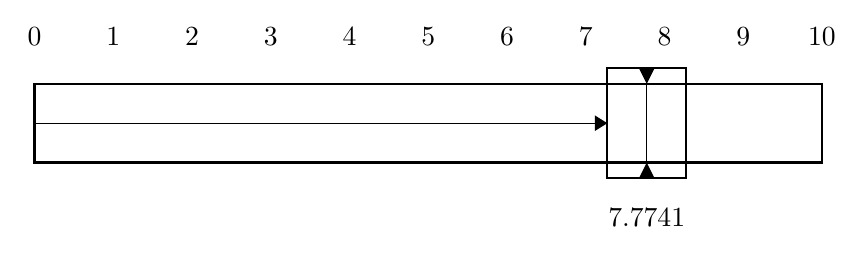
\begin{tikzpicture}
            % Ruler
            \draw [thick] (0,0) rectangle (10,1);
            \draw (0,0.5) -- ++(7.2741,0);
            \fill (7.2741,0.5) -- ++(-0.16,0.1) -- ++(0,-0.2);
            \foreach \i in {0,...,10} {
                    \draw (\i,1.6) node {$\i$};
            }
            
            % Slider
            \draw [thick] (7.2741,-0.2) rectangle (8.2741,1.2);
            \draw (7.7741,-0.2) -- (7.7741,1.2);
            \fill (7.7741,0) -- ++(-0.1,-0.2) -- ++(0.2,0);
            \fill (7.7741,1) -- ++(-0.1,0.2) -- ++(0.2,0);
            \draw (7.7741,-0.7) node {$7.7741$};
        \end{tikzpicture}
    \end{center}
    \vspace{4mm}
        
    Any digital encoding of numbers is possible in computing, and the choice does not affect what a computer theoretically can or cannot do. Rather, it has practical consequences. Decimal encoding was implemented in a number of early electronic and electro-mechanical computers, such as the Harvard Mark I and the ENIAC. 

\end{bluebox}

Regardless of which encoding is used, data is data.

Data are unorganized facts or statistical values that may reveal something of interest. They are collected by \textit{sampling} the properties of \textit{phenomena} from the observable Universe. Once collected, they can be cleaned, organized, and then analyzed in the hope of gaining a better understanding of reality. When a set of structured data is put into context, it can be interpreted as \textit{information} that explains what has been observed. This information can then be \textit{encoded} as an ordered sequence of data known as a \textit{message}. Messages are \textit{transmitted} and \textit{received} both by Nature and by Man. In the latter case, this process can be viewed as the \textit{communication} of abstract, human thought.

Data can describe a variety of things, such as quantities, qualities, and relations. In computer science, data are \textit{quantitative}. That is, they describe \textit{quantities}, which are properties that can be modeled with \textit{numbers}. A quantity can be further classified as either a \textit{multitude} or a \textit{magnitude}. The former is a \textit{discrete} quantity that is \textit{counted}. One would ask "how many" elements belong to a multitude. In contrast, a magnitude is a \textit{continuous} quantity that is \textit{measured}. It is the size of something that is modeled as a \textit{continuum} (e.g. by fields such as $\mathbb{R}$ or $\mathbb{C}$), and one would accordingly inquire as to "how much" of it there is.

A set of data collected at a finite rate (e.g. by a \textit{measuring instrument}) is technically a  multitude of samples, even if the quantity being measured is a magnitude. For example, if a ball were thrown in the air, one could ask "how much" height it has at regular intervals of time. Once the data collection ends, one can also ask "how many" samples were acquired. Furthermore, one can ask "how often" samples were taken. This is an evaluation of the \textit{sampling rate}, and it is really just an alternative way of asking with "how much" speed samples were taken. Rates and ratios are still quantities. The existence of the rational numbers $\mathbb{Q}$ are evidence enough of this.

Data can be represented by various \textit{media}, both symbolic and physical. In the age of modern computing, data are often assumed to be \textit{digital} in nature, expressed in the symbolic medium of numerical \textit{digits}. This is the case for data processed by modern, electronic computers, which charge capacitors in order to generate voltages that represent \textit{logic levels}. A \textit{transistor} acts as a gate to each capacitor, staying closed to retain \textit{electric charge} during storage and opening to measure or modify voltage on reads and writes respectively.

The ratio of a capacitor's charge to its capacitance determines its voltage (i.e. $V=\frac{q}{C}$). This voltage is then mapped to a logic level, which corresponds to a range of voltage values. These logic levels represent digits. In modern computer memory, data are represented as binary digits or \textit{bits} (i.e. the digits 0 and 1), each of which represents a binary number. In this case, there are two logic levels, \textit{low} and \textit{high}.

\begin{table}[H]
    \centering
    \caption{Voltage Ranges for CMOS Logic Levels (V)}
    \label{tab:logiclevels}
    \begin{tabular}{|c|c|c|}
        \vtabularspace{3}
        \hline
        Signals & Low (0) & High (1) \\
        \hline
        Input & 0.00--1.50 & 3.50--5.00 \\
        Output & 0.00--0.05 & 4.95--5.00 \\
        \hline
    \end{tabular}
\end{table} 

However, quantitative data need not be expressed with symbolic digits. They can instead be defined in terms of an \textit{analogous} physical quantity. For example, the unit of measurement known as the \textit{millimeter of mercury} (mmHg) defines pressure in terms of the height of a column of mercury in a manometer. It is used to quantify blood pressure, and it does so by considering height an \textit{analog} or \textit{model} of pressure measuring that instead. Using this method, data about one phenomenon can be encoded as data of a different phenomenon, provided that the quantities involved are somehow related to each other. In this case, a height of 1 mm is related to a pressure of 133.322 Pa above atmospheric pressure.

\section{Semiotics, Language, and Code}

However, the term "universal language" is also often used in other contexts to describe a hypothetical language that all of the world speaks and understands. This is an old idea, and it is addressed in a number of myths and religious texts. In Genesis, the myth of the Tower of Babel explains the diversity of language as a result of God thwarting the Babylonians' plan to build a tower that would extend into the heavens. As punishment for their blasphemy, God "confused their tongues" and dispersed them across the world, shattering their once universal language. Similar myths are told by cultures across the world, such as the Native American Tohono O'odham people, who tell tales of Montezuma attempting to do the same, attracting the ire of the Great Spirit.

Alas, no such language exists and it is unlikely that one has ever existed. Rather, human language is generally believed to have evolved independently around the world from prelinguistic systems of communication such as gesturing, touching, and vocalization about 100,000 years ago. Similarly, written language evolved from proto-writing, the repeated use of symbols to identify objects or events.

Writing is distinct from speaking in that it is a reliable method of storing and transmitting information. Before the invention of written language, important pieces of history and literature were preserved through \textit{oral tradition}, passing from one generation to the next through repetition and memorization. However, oral tradition is prone to data loss and unintended changes. Like messages in a game of telephone spanning centuries, stories were at risk of losing old details and gaining extraneous ones. Additionally, if a society fell apart, their stories could be lost forever. Writing is a tool that mitigates these issues by \textit{encoding} speech into a symbolic code that can be inscribed onto durable media, such as clay tablets or stone, or onto more delicate, portable media such as parchment or paper.

\subsection{Writing Systems}

A \textit{symbol} is a syntactic mark that is understood to represent a semantic idea. For example, the numeral "$2$" is a symbol for the abstract concept of the number known as "two," the quantity of items in a pair. Symbology is universal for mankind, as it is an exercise of our capacity for abstract thought. Humans can leverage the pattern-recognizing power of the brain to associate symbols or sequences of symbols (also known as \textit{strings}) with ideas. Thus, we can proliferate information textually by means of a \textit{writing system}.

$\cdots$

An argument of any kind must be expressed in a \textit{language}. In the case of an informal argument, such as a debate, a \textit{natural language} is typically used (i.e. a language, spoken or written, that evolved \textit{naturally} as an aspect of human culture). This is done in the name of \textit{universality}. For example, a political debate that is held and perhaps broadcast in Poland would likely be conducted in Polish because Polish politics are primarily of interest to Polish people. Many Poles speak English in addition to Polish, but there is no language more widely spoken in Poland than Polish, with a whopping 97\% of the country declaring it as their first language. For media directed toward the population of Poland, there is no language that will better ensure an effective dissemination of ideas. It is a nearly \textit{universal} language in this context, a language understood by all intended recipients.

Formal proofs, on the other hand, require a \textit{formal language} for clarity and precision. In practice, formal proofs are rarely written or read by logicians or mathematicians. Typically, mathematical proofs are written using a combination of formal and natural language. However, computer programs, written in \textit{programming languages}, are considered formal.

A formal language is constructed from an \textit{alphabet} $\Sigma$, which is a set of symbols. The set of all possible finite-length \textit{words} or \textit{formulas} that can be built from this alphabet is denoted $\Sigma^*$. A formal language $L$ over an alphabet $\Sigma$ is then defined as a subset of $\Sigma^*$. Thus, a language is a set of purely syntactic objects. It may conform to a \textit{grammar} that specifies how words can be produced or arranged in a \textit{sentence}, but a language is never inherently meaningful. The semantics of a language is always interpreted separately from the syntax.

\subsection{Numeral Systems}


\chapter{Logic and Mathematics}

\vspace{4mm}
\begin{displayquote}
    \textit{Upon this first, and in one sense this sole, rule of reason, that in order to learn you must desire to learn, and in so desiring not be satisfied with what you already incline to think, there follows one corollary which itself deserves to be inscribed upon every wall of the city of philosophy:
    \vspace{1mm}
    \begin{center} Do not block the way of inquiry. \end{center}}
    \vspace{2mm}
    \begin{flushright}
        ---Charles Sanders Peirce
    \end{flushright}
\end{displayquote}
\vspace{3mm}

\section{The Syntax and Semantics of Argument}

\textit{Reasoning} is a cognitive act performed by rational beings. It involves the absorption and synthesis of presently available information for the purpose of elucidating knowledge. It may require the ingenuity of thought, but in some cases the rote application of simple rules is sufficient. Reasoning could also be described as the providing of good \textit{reasons} to explain or justify things. However, as you might expect, there is much debate over whether or not any particular reason is "good." Reasoning is broad, and it comes in different flavors, but ultimately it is the pursuit of \textit{truth}. \\

Reasoning may involve the application of \textit{logic}. This \textit{logical reasoning} is the kind of reasoning that can be expressed in the form of an \textit{argument}. However, this argument does not need to be "correct." Such reasoning simply must be explainable in \textit{steps}, whether that be through informal speech or formal writing. \\

In logic, an argument has two parts: a set of two or more \textit{premises} and a \textit{conclusion}. If the conclusion \textit{necessarily} follows from the premises, the argument is called \textit{valid}. To know whether or not an argument is valid, one must produce a step-by-step \textit{deduction} of the conclusion from its premises. \\

A deduction is constructed within a \textit{deductive system}, which also has two parts: a set of two or more \textit{premises} and a set of \textit{rules of inference}. A rule of inference can be thought of as a kind of logical function. It takes statements (such as premises) as input and outputs either an intermediate result or the conclusion. A deduction, then, has \textit{three} parts: a set of two or more \textit{premises}, a \textit{conclusion}, and a set of \textit{intermediates}. A single-step deduction is represented below, along with a suitable rule of inference labeled $MP$. Note that the set of intermediates is empty in the case of deductions with only one step. \\[2mm]

% Modus Ponens diagram
\begin{center}
    \begin{tikzpicture}[scale=0.2]
        \tikzstyle{every node}+=[inner sep=0pt]

        \draw [black] (0,0) circle (3);
        \draw (0,0) node {$P$};
        
        \draw [black] (15,0) circle (3);
        \draw (15,0) node {$Q$};
        
        \draw [black] (3,0) -- (12,0);
        \fill [black] (11.2,0.5) -- (11.2,-0.5) -- (12,0);
        
        \draw [black] (0,-10) circle (3);
        \draw (0,-10) node {$P$};
        
        \draw [black, thick] (-9,-17) -- (18,-17);
        
        \draw [black] (0,-24) circle (3);
        \draw (0,-24) node {$Q$};
        
        \draw (-7,0) node {$1^\textit{st}$};
        \draw (-7,-10) node {$2^\textit{nd}$};
        \draw (-7,-24) node {$\textnormal{Con.}$};
        
        %----------------------------------------
        
        \draw [very thick] (26,3) rectangle (48,-27);
        \fill [textbook-blue] (26.1,2.9) rectangle (47.9,-26.9);
        
        \draw (37,-6.5) node {\fontsize{50}{40} $\textnormal{M}$};
        \draw (37,-18.5) node {\fontsize{50}{40} $\textnormal{P}$};
        
        %----------------------------------------
        
        \draw [black, thick] (22,3.07) -- (22,-13.07);
        \draw [black, thick] (22,3) -- (21,3);
        \draw [black, thick] (22,-13) -- (21,-13);
        \draw [black, thick] (22,-5) -- (26,-5);
        \fill [black] (25.2,-4.5) -- (25.2,-5.5) -- (26,-5);
        
        \draw [black, thick] (22,-20.93) -- (22,-27.07);
        \draw [black, thick] (22,-21) -- (21,-21);
        \draw [black, thick] (22,-27) -- (21,-27);
        \draw [black, thick] (22,-24) -- (26,-24);
        \fill [black] (22,-24) -- (22.8,-23.5) -- (22.8,-24.5);
    \end{tikzpicture}
\end{center}
\vspace{5mm}

This is the quintessential rule of inference used in logical reasoning, expressed here in symbols. It is known as \textit{modus ponens} (Latin for "a method that affirms"). The first premise $P\rightarrow Q$ is called a \textit{conditional statement} where $\rightarrow$ is the \textit{implies} operator. It states that if the \textit{antecedent} $P$ were true, it would \textit{imply} that the \textit{consequent} $Q$ would also be true. The second premise $P$ simply states that the statement $P$ is indeed true. Thus, by means of \textit{modus ponens}, we can \textit{infer} from the premises $P\rightarrow Q$ and $P$ that the conclusion $Q$ must be true. \\

Inference is also called \textit{entailment}. Though these terms describe the same logical concept, the latter more aptly describes the relationship between statements that are connected in a deduction. To infer is to come to a conclusion that is not \textit{explicitly} stated in the premises. To entail is to require that something follows. If $P$ \textit{entails} $Q$, this suggests that $Q$ is a \textit{logical consequence} of $P$, which we can express using a \textit{turnstile}: $P\vdash Q$. Inference is an action that humans perform. Entailment is a relationship between logical rules. \\

When the inferences made mirror the entailment, you've got yourself a \textit{valid} argument. However, this does not necessarily mean that your argument is \textit{sound}. \textit{Validity} is a property of arguments with a conclusion that can be \textit{deduced} from its premises according to rules of inference. However, validity says nothing about whether or not the premises have a \textit{meaning} that accurately describes reality. \textit{Soundness}, on the other hand, is a property of valid arguments whose premises are \textit{known truths} or \textit{axioms}. The deduction of a sound argument is called a \textit{proof}. \\

Validity and soundness complicate entailment. Now, an argument can be evaluated either in terms of its \textit{syntax} or in terms of its \textit{semantics}. Syntax refers to the arrangement of symbolic \textit{words} (or, more generally, \textit{tokens}) in a body of text. Semantics, on the other hand, refers to the \textit{meaning} that can be \textit{interpreted} from the text. Both of these concepts are integral to human language and indeed to the communication of information in general. \\

Consider the following valid deduction: \\

\begin{center}
    \begin{tabular*}{0.55\textwidth}{@{\extracolsep{\fill} } ll}
        \textnormal{"If it is raining, it is Tuesday."} & $P\rightarrow Q$ \\
        \textnormal{"It is raining."} & $P$ \\
        \hline
        \textnormal{"Therefore, it is Tuesday."} & $\therefore Q$ \\
    \end{tabular*}
\end{center}
\vspace{4mm}

This conclusion is a \textit{syntactic consequence} of the premises ($P\vdash Q$). That is, when the argument is evaluated simply as a collection of symbolic strings that are manipulated according to rules, $P$ entails $Q$. \\

Syntactic consequence is sometimes expressed with the following statement: "If the premises are true, the conclusion must also be true." However, while this statement does hold for all valid arguments, text evaluated syntactically does not have any notion of truth. It is simply a sequence of tokens. Thus, it may be better to think of valid arguments as "games that are played according to the rules." For example, chess has no inherent meaning associated with it, but it still has rules, and valid games of chess are those that comply with those rules. \\

Now, it might be Tuesday and raining as you are reading this. However, semantically, it is not required to be Tuesday if it is raining. The first premise given above is, in reality, false. However, if we change it to something that we consider true, we can come to a conclusion that is both valid and sound: \\

\begin{center}
    \begin{tabular*}{0.55\textwidth}{@{\extracolsep{\fill} } ll}
        \textnormal{"If it is raining, it is wet outside."} & $P\rightarrow Q$ \\
        \textnormal{"It is raining."} & $P$ \\
        \hline
        \textnormal{"Therefore, it is wet outside."} & $\therefore Q$ \\
    \end{tabular*}
\end{center}
\vspace{4mm}

In this case, the conclusion is a \textit{semantic consequence} of the premises ($P\vDash Q$). In addition to the argument being syntactically logical, it is also semantically true "in all universes." That is, there is no possible scenario where it is raining, and it is not wet outside. This syntactic-semantic difference will come up repeatedly throughout this guide. \\

\section{The Structure of Proof}

Of course, arguments can have more than one step. An argument can involve many inferences, some of which may use \textit{intermediate conclusions} as premises for further conclusions. Multiple threads of reasoning can extend from the premises, weaving through intermediate conclusions and intertwining via inference until they all meet at a \textit{final conclusion}. This is the \textit{tree structure} that is inherent in a \textit{formal proof}. \\

% Tree Structure of Proofs
\begin{center}
    \begin{tikzpicture}[scale=0.2]
        
        \coordinate (L) at (135:10);
        \coordinate (R) at (45:10);
        
        % Level 0
        \draw [black] (0:0) -- ++(L);
        \draw [black] (0:0) -- ++(R);
        
        \fill [white] (0:0) circle (3);
        \draw [black] (0:0) circle (3);
        \draw (0:0) node {$F$};
        
        % Level 1
        \draw [black] (R) -- ++(L);
        \draw [black] (R) -- ++(R);
        
        \fill [white] (L) circle (3);
        \draw [black] (L) circle (3);
        \draw (L) node {$P_1$};
        
        \fill [white] (R) circle (3);
        \draw [black] (R) circle (3);
        \draw (R) node {$I_2$};
        
        % Level 2
        \draw [black] ($ 2*(R) $) -- ++(L);
        \draw [black] ($ 2*(R) $) -- ++(R);
        
        \fill [white] ($ (R) + (L) $) circle (3);
        \draw [black] ($ (R) + (L) $) circle (3);
        \draw ($ (R) + (L) $) node {$P_2$};
        
        \fill [white] ($ 2*(R) $) circle (3);
        \draw [black] ($ 2*(R) $) circle (3);
        \draw ($ 2*(R) $) node {$I_1$};
        
        % Level 3
        \fill [white] ($ 2*(R) + (L) $) circle (3);
        \draw [black] ($ 2*(R) + (L) $) circle (3);
        \draw ($ 2*(R) + (L) $) node {$P_3$};
        
        \fill [white] ($ 3*(R) $) circle (3);
        \draw [black] ($ 3*(R) $) circle (3);
        \draw ($ 3*(R) $) node {$P_4$};
        
        % Arrows        
        \foreach \i in {0,1,2} {
                \coordinate (A) at ($ (45:3) + \i*(R) $);
                \coordinate (B) at ($ (135:3) + \i*(R) $);
                \fill [black,rotate around={45:(A)}] (A) -- ++(0.8,0.5) -- ++(0,-1);
                \fill [black,rotate around={45:(B)}] (B) -- ++(-0.5,0.8) -- ++(1,0);
        }
        
    \end{tikzpicture}
\end{center}
\vspace{4mm}

In this \textit{tree}, the \textit{first premises} are labeled as $P_n$ where $n\in\{1,2,3,4\}$, the \textit{intermediate conclusions} are labeled as $I_m$ where $m\in\{1,2\}$, and the \textit{final conclusion} is labeled $F$. Though one can make a distinction between first premises and intermediate conclusions, it is important to note that they are all premises with regard to the eventual final conclusion. Thus, there are no restrictions on combining them beyond those dictated by the rules of inference. \\

In modern proof theory, proofs like these are studied not only for their semantic meaning, but also for their mathematical structure. They are treated like \textit{data structures}, which are abstract objects that are used in computer science to model the storage and flow of digital \textit{information}. Similarly, a proof is an abstract text that models the flow of logical information as it is manipulated by rules of inference toward a final conclusion. \\

Information, in the context of computer science and, more generally, \textit{information theory}, refers to a \textit{syntactic} message. Formally, it is an order sequence of symbols \\

In computer science, the data structures of interest are \textit{recursive}. That is, the structure can be defined "in terms of itself." \textit{Recursion} is a deep topic, and we will spend much of the next part characterizing it, but a practical way to think about a recursive structure is in terms of \textit{type}. \\

Types are a widespread feature in programming languages. As a concept, they are founded in a logical system called a \textit{type theory}. There are multiple type theories, and some of them are used as alternative foundations for mathematics. We will cover all of this in detail later, but, essentially, a type is a label that can be given to 

However, not all forms of reasoning have such strict rules. There are other methods of reasoning that cannot be modeled by an argument. In contrast to logical reasoning, \textit{intuitive reasoning} has steps that are \textit{not} understood. Although the question might seem peculiar, it is worth asking whether or not computation can be intuitive. So, to begin our journey of understanding computation in a modern, logical sense, we will first walk in the other direction, considering it instead in a mystical, otherworldly sense. \\

\section{Intuitive Reasoning: The Oracle, the Seer, and the Sage}

\textit{Intuition} is the capacity to create conclusions without evidence, proof, or a combination of the two. If any premises are involved, they may appear to an onlooker as if they were plucked out of thin air. If any method is involved, it is esoteric or hidden from sight. Acts of intuition range from the mundane procedures we perform without thinking to great feats of intellectual, artistic, and athletic achievement. And while it is often associated with magic or supernatural ability, intuition is a real, observable phenomenon, and it is a form of reasoning. \\

Like that of reasoning, the definition of intuition is fuzzy. There are a variety of events that one might label as the product of intuition that are actually quite functionally distinct from one another. For this reason, I would like to consider and compare three archetypes that are known for their intuitive skills: the Oracle, the Seer, and the Sage. For the skeptics among you, I ask that you suspend your disbelief for a moment and assume that our characters are acting in good faith. There is no lying here; the conclusions are sincere. \\

\paragraph{The Oracle} \hspace*{1mm} \vspace*{2mm}

An Oracle is a person who predicts the future by acting as a vessel for a god or a set of gods. They are considered by believers to be portals through which the divine speaks directly. They are found in histories all over the world, but most people associate the role with the priestesses of Ancient Greece. Picture a woman with eyes that roll back into her head as she speaks in a possessed, thundering voice. \\

For an Oracle, the conclusions come straight from the source. She may not even do any reasoning herself, save for the \textit{unconscious reasoning} that is performed while she is possessed. However, conscious or not, she provides a great service to mankind. There is no clearer answer than the one given to you directly from the gods themselves, even if it has to be sent through what is essentially the human version of a telephone. \\

For those seeking counsel, the premises of the Oracle's conclusion are unnecessary because they just \textit{know} that the statement must be true. For them, the connection the Oracle has with the gods and with reality is part of life itself. We all have deep beliefs like this. For example, most people do not feel that gravity needs to be proven to them in order for them to accept it as fact. Their perception of gravity in the world around them is proof enough. This is the kind of intuition characterized by \textit{subconscious reasoning}, the reasoning you do without being aware of doing it. \\

\paragraph{The Seer} \hspace*{1mm} \vspace*{2mm}

A Seer is a person who predicts the future by interpreting signs from a god or a set of gods. Unlike an Oracle, a Seer speaks divine truth in his own words, drawing from an innate, sometimes god-given power to see meaning in natural events or occult objects. There are various methods of divination that are used by Seers, such as scrying (the gazing into magical things, like crystal balls, for the purpose of seeing visions), auspicy (the interpretation of bird migration), or dowsing (the use of magic to find water, often with the aid of a dowsing rod). The acceptance of any particular method is cultural, but beliefs in divination vary greatly, even within a single society. \\

The Seer has premises for his conclusion, but the rules of inference involved in his reasoning are incomprehensible to others. He 

\paragraph{The Sage} \hspace*{1mm} \vspace*{2mm}

\begin{tcolorbox}[breakable, enhanced, colback=textbook-blue, sharp corners]
    \vspace{3mm}
    \begin{center}
        \textbf{What is Truth?}
    \end{center}
    Truth, in the absolute sense, has been discussed and debated since the dawn of man. It is a concept that seems obvious to us, and yet it always seems to elude our understanding. Philosophers have formulated dozens of theories of truth over the years, with some asserting that truth is an objective property of our universe and others asserting that truth is a useful lie that mankind has invented. And while there is merit in those claims that truth is not real, we still see around us the technology that was born out of our intuitive sense of true and false. Especially in computer science where everything is represented in binary. \\

    The traditional theories of truth have been termed \textit{substantive}. That is, they assert that truth has some basis in reality and that it is a meaningful thing to discuss. Early theories of truth from Ancient Greece are considered the foundation of \textit{correspondence theory}, the idea that statements are true if their symbols are arranged in such a way that they express an abstract thought that accurately describes reality. This theory defines truth in the context of a relationship between language and objective reality. It is a useful philosophy that allows us to orient ourselves in the world around us. However, many philosophers believe that truth cannot be explained by such a simple rule. In fact, there are many more factors that could play a role in the concept. \\

    Objections to a strict correspondence theory usually take issue with the treatment of language as something monolithic and easy to classify within a true-false dichotomy. For example, a statement encoded as a sentence in a language is only meaningful to people who can read that language. What does this imply about a particular language's relationship with truth? Is a statement only true for those who understand it? Furthermore, there is no guarantee that readers of the same language will even be able to agree on the meaning expressed by a particular sentence. Languages often encompass multiple dialects that might parse words differently. Words themselves also may not be precise, and some abstract thoughts may not have suitable words in some languages. These are the points raised in \textit{social constructivism}, a theory which avers that human knowledge is historically and culturally specific. Social constructivists also believe that truth is \textit{constructed} and that language cannot faithfully represent any kind of objective reality. \\

    Other substantive theories find the essence of truth nestled in other abstract concepts. \textit{Consensus theory}, as the name implies, defines truth as something that is agreed upon either by all human beings or by a subset (such as academic groups or standards bodies). This is another anthropocentric definition that is at constant risk of philosophical division on any given topic. \textit{Coherence theory} takes a more objective approach, claiming that a statement can only be true if it fits into a system of statements that support each other's truth. This is similar to the notion of \textit{formal systems}, which we will discuss in depth later. However, traditional coherence theories attempt to explain all of reality within a single coherent system of truths, which is incompatible with our modern understanding of formal systems. \\

    Modern developments in philosophy have resulted in theories that deviate from the long-held, substantive opinions on the nature of truth. These \textit{minimalist} theories assert instead that truth is either not real or not a necessary property of language or logic. They claim that statements are \textit{assertions} and thus are implicitly understood to be true. For example, it is understood that by putting forth the sentence "$2+2=4$," you are endorsing the semantic meaning "$2+2=4$ is true." The clause "is true" is called a \textit{truth predicate}, and minimalist theories of truth often consider its use redundant. \\

    This idea of a truth predicate is borrowed from Alfred Tarski's \textit{semantic theory of truth}, which is a substantive theory that refines the correspondence concepts espoused by Socrates, Plato, and Aristotle for formal languages. This theory makes a distinction between a statement made in a formal language and a truth predicate, which evaluates the truth of the statement. Tarski made this distinction in order to circumvent the \textit{liar's paradox}, which is often presented with the following example: "This sentence is false." If the predicate "is false" is considered to be part of "this sentence," the truth of this statement cannot be decided. For this reason, Tarski states that a language cannot contain its own truth predicate. This is enforced by requiring that "this sentence" be written in an \textit{object language} and that "is false" be written in a \textit{metalanguage}. \textit{Convention T}, the general form of this rule, can be expressed as

    \begin{center}
        \textit{"$P$" is true if and only if $P$}
    \end{center}
        
    where "$P$" is simply the metalanguage sentence $P$ rendered in the object language. That is, the \textit{syntactic representation} is assigned a \textit{truth value} of true if and only if the semantic meaning it represents is considered true (according to whatever theory of truth you employ). By this rule, we say that "$2+2=4$" is true if and only if \textit{the sum of the number $2$ with the number $2$ is equal to the number $4$}. Minimalist redundancy theories modify Tarski's theory by interpreting "$P$" as an implicit assertion of the truth of $P$. The sentence "$P$," which asserts that $P$ is true, is then false if and only if its semantic meaning $P$ is false. \\

    \parbreak

    The debate on the nature of truth rages on \textit{in perpetuum}. However, for our purposes, we must be practical. There is truth in logic and mathematics and computer science as well, but, in practice, it has little to do with the debates on \textit{absolute truth} described above. Their truth is \textit{relative}. That is, it relies on the assumption that our premises are true. Cognizant of this, we move forward with our thinking, searching for truths within these arbitrary boundaries. \\
    \vspace{3mm}
\end{tcolorbox}
\vspace{2\baselineskip}

\section{Logical Reasoning: The Mathematician, the Scientist, and the Detective}

Logical reasoning is the \textit{inference} of new information from present information. It involves \textit{rule of inferences} that are used to relate sets of \textit{premises} to \textit{conclusions}. There are three kinds of logical reasoning: \textit{deductive}, \textit{inductive}, and \textit{abductive}. Each is classified according to which piece of information (premises, rule, or conclusion) is missing and must be inferred from the others. \\

Inductive arguments exist on a spectrum between \textit{weak} and \textit{strong}. Those that are stronger and more persuasive have a higher probability of having a true conclusion. Inductive reasoning is associated with \textit{science} and \textit{critical thinking} because it allows one to make generalizations about complex phenomena given limited evidence. Unlike deductive reasoning, it attempts to find new knowledge that is not simply contained within its premises. \\

Statements made by induction are bolstered with evidence whereas deductive statements are as true as their premises. This leaves inductive reasoning susceptible to \textit{faulty generalizations} and \textit{biased sampling}. Induction must also assume that future events will occur exactly as they have in the past, which is not always the case. For example, a turkey that is fed every morning with the ring of a bell may infer by induction that bell $\rightarrow$ food. However, he will see the error in his reasoning when the farmer rings the bell on Thanksgiving Day and instead slits his throat. \\

\paragraph{Abductive Reasoning} \hspace*{1mm} \vspace*{2mm}

\textit{Abductive reasoning} is the inference of a \textit{premise}, given a conclusion and a rule. It is investigative in nature. For example, given a conclusion "The grass is wet" and a rule "When it rains, the grass gets wet," we might determine that rain is the best explanation for the wetness of the grass. Thus, we abduce that "It might have rained." \\

Like induction, abduction can also produce a hypothesis. However, abduction does not seek a new relationship between two previously unconnected statements. Rather, it uses established relationships to find a reasonable explanation for a statement that is assumed to be true. It is often used by detectives or diagnosticians who need to find a probable cause of an event. It is also used in Bayesian statistics. While multiple premises may be abduced, typically we want to abduce a single, "best" premise. \\

Abductive reasoning allows us to ignore the many causes that are unlikely in favor of those few that may be relevant to the problem at hand. For example, doctors are often taught to heed the following proverb: "When you hear hoofbeats, think of horses, not zebras." That is, when a patient exhibits certain symptoms, a doctor should abduce from them a commonplace disease before considering more exotic possibilities. However, "zebras" do exist. Sometimes the most likely cause is not the actual cause. For this reason, abduction is also considered to be equivalent to a deductive fallacy called \textit{affirming the consequent}, which is like a \textit{modus ponens} performed in reverse. That is, given a conditional $P\rightarrow Q$ and the consequent $Q$, abduction infers $P$ from $Q$ by assuming that the converse $Q\rightarrow P$ of the conditional is also true. This is not a deductively valid inference. Considering our example again, the grass might be wet from rain, but this is not \textit{necessarily} true. It is also possible that the sprinkler system is on. Or perhaps there is a zebra-esque scenario like a flood. \\\\



% Dinkus

% Conclusion to Volume I
What is the strange loop? What is wisdom?

